\section{ODRL profile for Access Control}
\label{sec:oac}

This Section describes the development of OAC, an ODRL profile for Access Control, to express access policies associated with data stored in decentralised datastores.

\subsection{Profile requirements specification}
\label{sec:oac_requirements}

This Section outlines the motivation and identified requirements for the development of the OAC profile.
As previously mentioned, personal datastores, such as Solid Pods, need to deal with GDPR's requirements, particularly the information requirements set out in Articles 13 and 14, such as the identity of the controller, the purpose for processing, the personal data categories being processed, or the legal basis being used, if they are to be adopted as a legally compatible solution for the sharing of personal data in Europe.
Taking Solid as a use case, this information can be given to Solid users by employing conventional methods, such as a notice provided through the data requester's website.
However, for individuals to control their data practices, the Solid Pod must also record this information so that the individual has the opportunity to:

\begin{enumerate}
    \item [(i)] inspect their personal data within an environment under their control;
    \item [(ii)] store it for accountability purposes;
    \item [(iii)] determine their data access preferences; and
    \item [(iv)] be assisted in enforcing said preferences.
\end{enumerate}

To achieve this, it is necessary to understand the provisions of the law regarding the information that needs to be provided, including the particular requirements of certain legal bases such as consent, and the forms of control that individuals want to have or the information they want to know in the context of the handling of their personal data.
Therefore, based on these considerations, the usage of ODRL and DPV is motivated by the following needs: 

\begin{itemize}
  \item[1.]Organisations need to:
    \begin{itemize}
      \item[a)]Specify machine-readable data handling policies, which should be accessible by users;
      \item[b)]Document provenance information related to their personal data processing activities, including notices and activity logs;
      \item[c)]Determine and fulfil applicable rights and obligations based on specific data protection laws or other contextual information, e.g., specific categories of personal data;
      \item[d)]Implement security measures by default and by design, specifically related to personal data access.
    \end{itemize}

    \item[2.]Users need to:
    \begin{itemize}
      \item[a)]Express human-centric data-sharing preferences, e.g., willingness to share a specific data type for non-profit research or to prohibit processing for profiling purposes;
      \item[b)]Specify broad permissions, e.g., allow data access for scientific research, or restrict third party data collection;
      \item[c)]Specify narrow permissions, e.g., allow access to phone contact details for a particular app, or deny access to a specific resource;
      \item[d)]Have a policy conflict strategy, e.g., generally deny access to location data, but include an exception for specific applications;
      \item[e)]Understand who is using which data categories, for what purposes, sharing it with whom, and under what legal basis.
    \end{itemize}
    
\end{itemize}

Moreover, taking into consideration the previously described motivation points, the following requirements can then be specified for the OAC profile:

\begin{itemize}
      \item[R1.]Support specifying user preferences as policies.
      \item[R2.]Incorporate vocabulary specifying or aligned to legal concepts.
      \item[R3.]Support specifying permissions and prohibitions at arbitrary granularity.
      \item[R4.]Support identifying and resolving conflicts based on scope.
      \item[R5.]Record policies used to authorise access to data.
      \item[R6.]Support querying policies and authorisations for introspection of data access.
\end{itemize}

As such, following the LOT methodology, these requirements are consolidated in the profile's ORSD available in Table \ref{tab:OAC_ORSD}.
As Solid's current access control mechanisms only partially implement R1, R3, and R5, OAC allows its users to declare not only granular permissive policies but also prohibitive policies, both aligned with legal requirements, which can be stored in their decentralised datastores for future inspection and can be used with additional constraints and contextual information.

\begin{table}[htbp]
\centering
\caption{Ontology Requirement Specification Document of the OAC profile.}
\label{tab:OAC_ORSD}
\scriptsize
\begin{tabular}{| l | l | l | l  | l | l | l |l| }
\hline
\multicolumn{8}{|c|}{\cellcolor[HTML]{A0A0A0}\textbf{ODRL Profile for Access Control}} \\ \hline
\multicolumn{8}{|c|}{\cellcolor[HTML]{EFEFEF}\textbf{1. Purpose}} \\ \hline
\multicolumn{8}{| p{12.0cm} |}{The purpose of this profile of ODRL is to support policies determining the access to personal data stored in decentralised storage environments, such as Solid Pods.} \\ \hline
\multicolumn{8}{|c|}{\cellcolor[HTML]{EFEFEF}\textbf{2. Scope}} \\ \hline
\multicolumn{8}{| p{12.0cm} |}{The scope of this profile is limited to the definition of an ODRL Profile for Access Control in decentralised settings. In particular, the introduced elements will serve one of these purposes: (i) define actions supporting the enforcement of current ACL verbs, (ii) define data protection-related actions and restrictions defined in GDPR, (iii) any vocabulary element to support policy patterns that can be anticipated to be common, and (iv) elements necessary to support the authorisation reasoning decision. } \\ \hline
\multicolumn{8}{|c|}{\cellcolor[HTML]{EFEFEF}\textbf{3. Implementation Language}} \\ \hline
\multicolumn{8}{| p{12.0cm} |}{RDF, RDFS} \\ \hline
\multicolumn{8}{|c|}{\cellcolor[HTML]{EFEFEF}\textbf{4. Intended End-Users}} \\ \hline
\multicolumn{8}{| p{12.0cm} |}{Developers of decentralised storage servers and applications, such as Solid servers and apps.} \\ \hline
\multicolumn{8}{|c|}{\cellcolor[HTML]{EFEFEF}\textbf{5. Intended Uses}} \\ \hline
\multicolumn{8}{| p{12.0cm} |}{
Use 1. Declaration of a policy by an individual storing personal data in a decentralised datastore, such as a Solid Pod. \newline 
Use 2. Request of data made by an entity, service or application to gain access to the data in different modalities. \newline
Use 3. Records of data access with transparent information related to the policy matching algorithm, including contextual information. 
 } \\ \hline
\multicolumn{8}{|c|}{\cellcolor[HTML]{EFEFEF}\textbf{6. Ontology Requirements}} \\ \hline
\multicolumn{8}{|c|}{\cellcolor[HTML]{EFEFEF}\textbf{a. Non-Functional Requirements}}    \\ \hline
\multicolumn{8}{| p{12.0cm} |}{
NFR 1. The profile is published online with HTML documentation, following W3C's specification format. } \\ \hline
\multicolumn{8}{|c|}{\cellcolor[HTML]{EFEFEF}\textbf{b. Functional  Requirements: Groups of Competency Questions}}  \\ \hline
\multicolumn{5}{|c|}{\cellcolor[HTML]{EFEFEF}CQG1. Related to access} & \multicolumn{3}{|c|}{\cellcolor[HTML]{EFEFEF}CQG2. Related to GDPR} \\ \hline %\multicolumn{4}{c|}{\cellcolor[HTML]{EFEFEF}}    \\ \hline
\multicolumn{5}{ | m{7cm} |}{
CQ1. Which policy type is being defined? \newline
CQ2. Which actions are defined in the policy? \newline
CQ3. Which data types are mentioned in the policy? \newline 
CQ4. Which policy constraints need to be fulfilled? \newline 
CQ5. Who are the parties intervening in the policy? \newline 
CQ6. Which is the conflict strategy of a policy? \newline 
CQ7. What are the contextual elements that need to be considered in the policy matching algorithm? } & 
\multicolumn{3}{ m{5cm} |}{
CQ8. Which information about personal data and its processing is necessary to have legally aligned policies? \newline 
CQ9. What identification information needs to be provided by the policy parties? \newline 
}\\ \hline
\end{tabular}
\vspace{-0.1in}
\end{table}

%For continued interoperability and adherence to the specification, the proposed extension to Solid’s ACL must ideally continue to implement existing functionality while incorporating the legal and user-centric requirements.

Lastly, it should be clear that OAC is \textbf{not dependent on Solid}, as it is not based on any Solid-specific vocabularies, and can be used in other decentralised data environments.
Nevertheless, throughout this Thesis, the use of OAC is demonstrated through the Solid ecosystem as it is an example of the implementation of a decentralised environment for the sharing of (personal) data that is based on the Semantic Web stack of technologies.

\subsection{Profile implementation}
\label{sec:oac_implementation}

This ODRL profile relies on DPV, for the invocation of legal concepts related to data protection and privacy, and ACL, for the expression of access mode operations, to specify complex permissions, prohibitions or duties over the access to personal data resources.

Moreover, OAC policies can be used to add a new layer to decentralised data systems -- a layer that is currently missing from the Solid ecosystem for instance -- that will come between the data and the access authorisation, e.g., ACL or ACP authorisations, layers in order to provide a richer access control mechanism to such systems.
As an access control mechanism's main goal is to determine access by users or software agents to digital resources, the entities generating and/or providing the data must able to express policies that satisfy their preferences, while users or software agents who wish to access said data must be able to define policies that describe their data handling activities. 
By using these policies in an algorithm to match incoming access requests for data, an agreement over the access to a certain resource or type of data can be defined and the decentralised data system can provide a fine-grained access control mechanism to its users.
As such, OAC reuses ODRL's \texttt{Offer} policies to express the conditions for access to personal data stored in decentralised data systems, e.g. Solid Pods, \texttt{Request} policies to express users or software agents' access requests and \texttt{Agreement} policies to describe the agreed conditions for access to the data. 
The three types of policies are defined below, according to their definition provided in the ODRL Vocabulary \& Expression 2.2 Recommendation specification \citep{iannella_odrl_vocab_2018}:

\begin{itemize}
    \item \textbf{Offer} -- Policy that proposes the assigner's rules over an asset and does not grant any privileges to assignees.
    \item \textbf{Request} -- Policy that proposes the assignee's rules over an asset and does not grant any privileges to any parties.
    \item \textbf{Agreement} -- Policy issued by an assigned that grants privileges to the assignee over an asset.
\end{itemize}

OAC's core concepts are illustrated in Figure~\ref{fig:oac_diagram} and Tables \ref{tab:profile_classes} and \ref{tab:profile_properties} specify the alignment between the ODRL, DPV, and ACL terms to ensure that their semantics are correctly interpreted by OAC implementers.

%Its core concepts are the Preference and Requirement policies, a new set of operators to constraint the defined Purposes, Recipients, Legal Basis, Technical and Organisational Measures, Technology and Identity Provider constraints (which will require the usage of DPV's taxonomies), new properties to specify policies for applications and services, Processing and Access actions, as well as Personal Data Categories, and Legal Entities.

\begin{figure}[htbp]
    \centering
    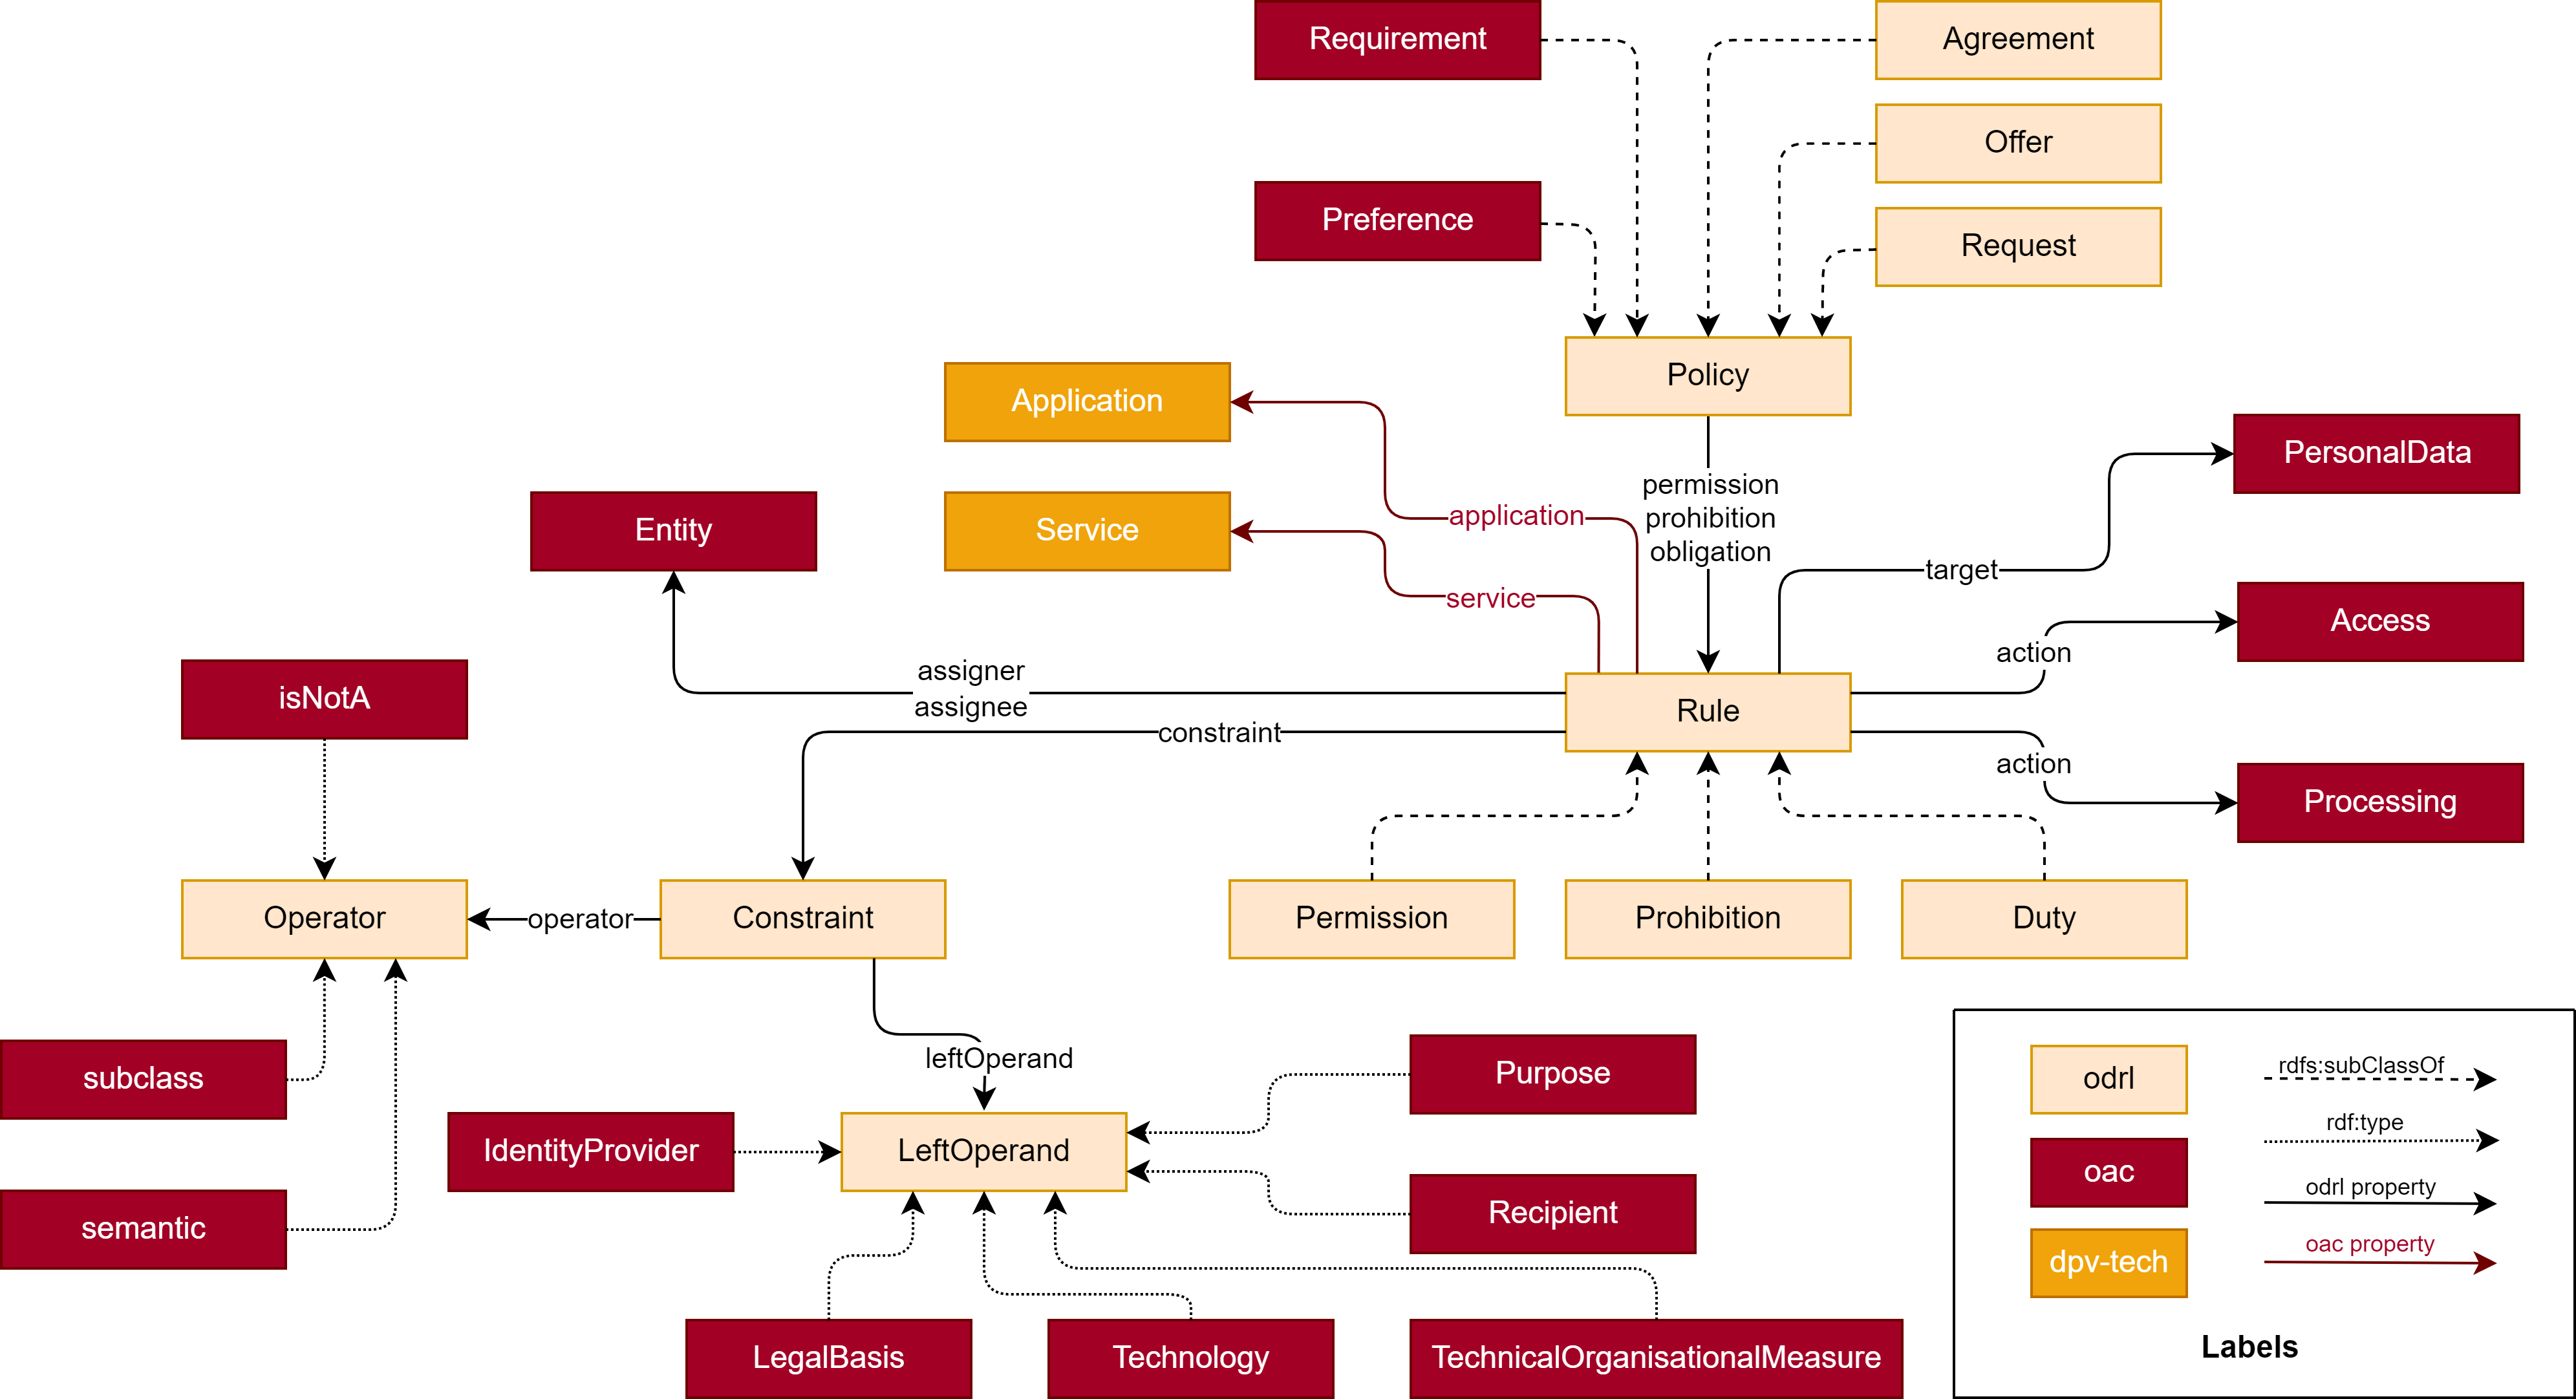
\includegraphics[width=\linewidth]{figures/chapter-4/oac_diagram.png}
    \caption{Diagrams of the concepts specified by the OAC profile.}
    \label{fig:oac_diagram}
\end{figure}

Two new types of policies, which can be combined in ODRL offers, are specified to deal with the preferences and requirements of users who wish to define rules for the processing of their personal data:

\begin{itemize}
    \item \textbf{Preference} -- Soft policy that expresses the assigner's preferences over a personal data asset which may not be satisfied and must not grant any privileges to assignees. If a preference policy set by party A does not match a request policy from party B, the request can still be accepted if party A accepts party B's request conditions.
    \item \textbf{Requirement} -- Hard policy that expresses the assigner's preferences over a personal data asset which must be satisfied and must not grant any privileges to assignees. If a requirement policy set by party A does not match a request policy from party B, the request must be denied even if party A accepts party B's request conditions.
\end{itemize}

\begin{table}[htbp]
\centering
\caption{Classes and named individuals specified in the OAC profile.}
\label{tab:profile_classes}
\resizebox{\textwidth}{!}{
\begin{tabular}{c||c|c}
Profile term & Instance of & Subclass of \\
\hline\hline
\texttt{oac:Preference} & & \texttt{odrl:Policy} \\
\hline
\texttt{oac:Requirement} & & \texttt{odrl:Policy} \\
\hline
\texttt{oac:isNotA} & \texttt{odrl:Operator} & \\
\hline
\texttt{oac:subclass} & \texttt{odrl:Operator} & \\
\hline
\texttt{oac:semantic} & \texttt{odrl:Operator} & \\
\hline
\texttt{oac:PersonalData} & \texttt{odrl:Asset} & \texttt{dpv:PersonalData} \\
\hline
\texttt{oac:Access} & \texttt{odrl:Action} & \texttt{acl:Access} \\
\hline
\texttt{oac:Processing} & \texttt{odrl:Action} & \texttt{dpv:Processing} \\
\hline
\texttt{oac:Entity} & \texttt{odrl:Party} & \texttt{dpv:Entity} \\
\hline
\texttt{oac:Purpose} & \texttt{odrl:LeftOperand} & \texttt{dpv:Purpose} \\
\hline
\texttt{oac:Recipient} & \texttt{odrl:LeftOperand} & \texttt{dpv:Recipient} \\
\hline
\texttt{oac:LegalBasis} & \texttt{odrl:LeftOperand} & \texttt{dpv:LegalBasis} \\
\hline
\texttt{oac:TechnicalOrganisationalMeasure} & \texttt{odrl:LeftOperand} & \texttt{dpv:TechnicalOrganisationalMeasure} \\
\hline
\texttt{oac:Technology} & \texttt{odrl:LeftOperand} & \texttt{dpv:Technology} \\
\hline
\texttt{oac:IdentityProvider} & \texttt{odrl:LeftOperand} & \\
\end{tabular}}
\end{table}

\begin{table}[htbp]
\centering
\caption{Properties specified in the OAC profile.}
\label{tab:profile_properties}
\begin{tabular}{c||c|c}
Profile property & Domain & Range \\
\hline\hline
\texttt{oac:service} & \texttt{odrl:Rule}, \texttt{odrl:Policy} & \texttt{dpv-tech:Service} \\
\hline
\texttt{oac:application} & \texttt{odrl:Rule}, \texttt{odrl:Policy} & \texttt{dpv-tech:Application} \\
\end{tabular}
\end{table}

Listing~\ref{list:oac_req_pref} presents an example of an OAC requirement and an OAC preference policies and Listing~\ref{list:oac_offer} an ODRL offer, based on the previously listed requirement and preference policies, as is indicated by the \texttt{dcterms:source} property.
The permission associated with the requirement policy contains the property \texttt{dpv:hasContext} associated with the term \texttt{dpv:Required} to indicate that said permission is a requirement, while the term \texttt{dpv:Optional} is used to identify the rules related with a preference policy.

\begin{listing}[htp]
\caption{OAC requirement and preference policies issued by \url{https://solidweb.me/besteves4/profile/card\#me}.}
\label{list:oac_req_pref}
\begin{minted}{turtle}
<https://solidweb.me/besteves4/policies/requirement1> a oac:Requirement ;
    odrl:uid <https://solidweb.me/besteves4/policies/requirement1> ;
    odrl:profile oac: ;
    dcterms:description "Requirement to read identifier data for identity verification purposes." ;
    dcterms:creator <https://solidweb.me/besteves4/profile/card#me> ;
    dcterms:issued "2023-10-20T18:22:15"^^xsd:dateTime ;
    odrl:permission [
        odrl:assigner <https://solidweb.me/besteves4/profile/card#me> ;
        odrl:target oac:Identifier ;
        odrl:action oac:Read ;
        odrl:constraint <#Constraint_Purpose_IdentityVerification> .

<#Constraint_Purpose_IdentityVerification> a odrl:Constraint ;
    dcterms:title "Purpose for access is to verify the identity of the assigner." ;
    odrl:leftOperand oac:Purpose ;
    odrl:operator odrl:isA ;
    odrl:rightOperand dpv:IdentityVerification .

<https://solidweb.me/besteves4/policies/preference1> a oac:Preference ;
    odrl:uid <https://solidweb.me/besteves4/policies/preference1> ;
    odrl:profile oac: ;
    dcterms:description "Preference to read age data if purpose is not commercial research." ;
    dcterms:creator <https://solidweb.me/besteves4/profile/card#me> ;
    dcterms:issued "2023-10-20T18:26:09"^^xsd:dateTime ;
    odrl:permission [
        odrl:assigner <https://solidweb.me/besteves4/profile/card#me> ;
        odrl:target oac:Age ;
        odrl:action oac:Read ;
        odrl:constraint <#Constraint_Purpose_not_CommercialResearch> .

<#Constraint_Purpose_not_CommercialResearch> a odrl:Constraint ;
    dcterms:title "Purpose for access is not commercial research." ;
    odrl:leftOperand oac:Purpose ;
    odrl:operator oac:isNotA ;
    odrl:rightOperand dpv:CommercialResearch .
\end{minted}
\end{listing}

\begin{listing}[htp]
\caption{ODRL offer issued by \url{https://solidweb.me/besteves4/profile/card\#me}.}
\label{list:oac_offer}
\begin{minted}{turtle}
<https://solidweb.me/besteves4/policies/offer1> a odrl:Offer ;
    odrl:uid <https://solidweb.me/besteves4/policies/offer1> ;
    odrl:profile oac: ;
    dcterms:description "Offer to read identifier data for identity verification and age data if purpose is not commercial research." ;
    dcterms:creator <https://solidweb.me/besteves4/profile/card#me> ;
    dcterms:source <https://solidweb.me/besteves4/policies/requirement1>, <https://solidweb.me/besteves4/policies/preference1> ;
    dcterms:issued "2023-10-20T22:15:34"^^xsd:dateTime ;
    odrl:permission [
        dpv:hasContext dpv:Required ;
        odrl:assigner <https://solidweb.me/besteves4/profile/card#me> ;
        odrl:action oac:Read ;
        odrl:target oac:Identifier ;
        odrl:constraint <#Constraint_Purpose_IdentityVerification>
    ] ;
    odrl:permission [
        dpv:hasContext dpv:Optional ;
        odrl:assigner <https://solidweb.me/besteves4/profile/card#me> ;
        odrl:action oac:Read ;
        odrl:target oac:Age ;
        odrl:constraint <#Constraint_Purpose_not_CommercialResearch>
    ] .

<#Constraint_Purpose_IdentityVerification> a odrl:Constraint ;
    dcterms:title "Purpose for access is to verify the identity of the assigner." ;
    odrl:leftOperand oac:Purpose ;
    odrl:operator odrl:isA ;
    odrl:rightOperand dpv:IdentityVerification .

<#Constraint_Purpose_not_CommercialResearch> a odrl:Constraint ;
    dcterms:title "Purpose for access is not commercial research." ;
    odrl:leftOperand oac:Purpose ;
    odrl:operator oac:isNotA ;
    odrl:rightOperand dpv:CommercialResearch .
\end{minted}
\end{listing}

Additionally, a set of three new ODRL operators, which are currently missing from the ODRL Core vocabulary Recommendation, and two new properties to specify policies applicable to certain services or applications, \texttt{oac:service} and \texttt{oac:application}, which are important stakeholders in decentralised data systems, are specified in OAC.
The newly introduced \texttt{oac:isNotA} operator is used in the \texttt{<\#Constraint\_Purpose\_not\_CommercialResearch>} constraint, in Listing~\ref{list:oac_req_pref}, to indicate that the purpose for access can not be an instance of the right operand of the constraint, e.g., \texttt{dpv:CommercialResearch}.
The \texttt{oac:subclass} operator can be used to indicate that a given left operand is a subclass of the right operand of the constraint, e.g., the purpose constraint of a rule can be a subclass of DPV's research and development purpose such as academic research, non-commercial research or commercial research, and the \texttt{oac:semantic} operator to express that a given left operand is equal to, an instance or a subclass of the right operand of the constraint, e.g., the purpose constraint of a rule can be research and development, an instance of research and development or one of its subclasses such as academic research, non-commercial research or commercial research.

Personal data is defined as an ODRL asset to define personal data-specific access policies, access modes and processing operations are defined as ODRL actions to define policies for specific access modes and/or processing operations which are not covered by ACL's access modes, e.g., \texttt{dpv:Transfer} or \texttt{dpv:Copy}, and DPV's \texttt{Entity} concept is defined as an ODRL party to define entity-specific access policies.
Additionally, when defining ODRL requests, the data requesters might use processing concepts, \texttt{dpv:Use, dpv:Collect, dpv:Share}, as the permitted/prohibited action of the rule that differ from the existing ACL's access modes, \texttt{acl:Read, acl:Write, acl:Append}.
As such, a mapping of ACL verbs to DPV processing operations is provided in OAC for such cases where offers and requests need to be matched and include both ACL access modes and DPV processing operations.
In this mapping, the \texttt{acl:Read} access mode corresponds to \texttt{dpv:Use, dpv:Collect} processing operations, and \texttt{acl:Write} resembles \texttt{dpv:Store, dpv:MakeAvailable}.
Furthermore, as previously mentioned, there are operations such as \texttt{dpv:Share} or \texttt{dpv:Transfer} that do not have a specific corresponding concept in WAC's ACL vocabulary, which require a greater introspection in the integration of legal processing concepts with access control operations.
Moreover, purposes, recipients, legal bases, technical and organisational measures, technologies and identity providers are defined as ODRL constraints to define constraint-restricted access policies.

Listing~\ref{list:oac_request} presents an example of an ODRL request that uses OAC terms and Listing~\ref{list:oac_agreement} an ODRL agreement which is the result of the matching between the offer defined in Listing~\ref{list:oac_offer} and the previously mentioned request.
In this example, Beatriz, identified by \url{https://solidweb.me/besteves4/profile/card#me}, and Arya, identified by \url{https://solidweb.me/arya/profile/card#me}, reach an agreement to allow read access operations over Beatriz's age data for the purpose of academic research in project X.
This \texttt{odrl:Agreement} is the result of the matching of \url{https://solidweb.me/besteves4/policies/offer1} and \url{https://solidweb.me/arya/requests/age_academicResearch}, as indicated by the \texttt{dcterms:references} property.
The legal basis of the agreement is consent, as is specified in the policy with the \texttt{dpv:hasLegalBasis dpv:Consent} terms, and Beatriz and Arya are registered as the data subject and data controller in question, respectively, using the \texttt{dpv:hasDataSubject} and \texttt{dpv:hasDataController} terms.
\beatriz{Policy matching and agreement generation is discussed in Chapter XX.}

\begin{listing}[ht]
\caption{ODRL request issued by \url{https://solidweb.me/arya/profile/card\#me}.}
\label{list:oac_request}
\begin{minted}{turtle}
<https://solidweb.me/arya/requests/age_academicResearch> a odrl:Request ;
    odrl:uid <https://solidweb.me/arya/requests/age_academicResearch> ;
    odrl:profile oac: ;
    dcterms:description "Request to read age data for academic research." ;
    dcterms:creator <https://solidweb.me/arya/profile/card#me> ;
    dcterms:issued "2023-10-21T13:47:56"^^xsd:dateTime ;
    odrl:permission [
        odrl:assignee <https://solidweb.me/arya/profile/card#me> ;
        odrl:action oac:Use ;
        odrl:target oac:Age ;
        odrl:constraint <#Constraint_Purpose_AcademicResearch>
    ] .

<#Constraint_Purpose_AcademicResearch> a odrl:Constraint ;
    dcterms:title "Purpose for access is to conduct academic research in project X." ;
    odrl:leftOperand oac:Purpose ;
    odrl:operator odrl:eq ;
    odrl:rightOperand ex:AcademicResearchProjectX .

ex:AcademicResearchProjectX a dpv:Purpose ;
    rdfs:subClassOf dpv:AcademicResearch ;
    rdfs:label "Conduct research in the academic project X." .
\end{minted}
\end{listing}

\begin{listing}[ht]
\caption{ODRL agreement to read age data for academic research based on consent.}
\label{list:oac_agreement}
\begin{minted}{turtle}
<https://solidweb.me/besteves4/policies/agreement1> a odrl:Agreement ;
    odrl:uid <https://solidweb.me/besteves4/policies/agreement1> ;
    odrl:profile oac: ;
    dcterms:description "Agreement to read age data for academic research based on consent." ;
    dcterms:creator <https://solidweb.me/besteves4/profile/card#me> ;
    dcterms:issued "2023-10-21T13:58:37"^^xsd:dateTime ;
    dcterms:references <https://solidweb.me/besteves4/policies/offer1>, <https://solidweb.me/arya/requests/age_academicResearch> ;
    dpv:hasDataSubject <https://solidweb.me/besteves4/profile/card#me> ;
    dpv:hasDataController <https://solidweb.me/arya/profile/card#me> ;
    dpv:hasLegalBasis dpv:Consent ;
    odrl:permission [
        odrl:assigner <https://solidweb.me/besteves4/profile/card#me> ;
        odrl:assignee <https://solidweb.me/arya/profile/card#me> ;
        odrl:action oac:Read ;
        odrl:target oac:Age ;
        odrl:constraint <#Constraint_Purpose_AcademicResearch>
    ] .
\end{minted}
\end{listing}

This Thesis focuses on \textit{Purpose, Personal Data, Processing, Recipients, Legal Bases, Technical and Organisational Measures} and \textit{Technologies} as the minimum `core concepts' for the OAC profile, and leaves out other DPV concepts such as rights or risks, which can be added at a later stage if needed.
Furthermore, similarly to WAC and ACP, OAC policies can also be defined for particular resources identified by URIs -- in such cases when an access request for a particular data type comes in, the authorisation mechanism must have information about what type of data those particular resources contain or else they will not be returned if they match the data type of the request.
Such information can be stored in a data registry, stored in a e.g. Solid Pod, where resources can be associated with the type of data they contain by using DPV's \texttt{hasPersonalData} property and DPV-PD's taxonomy of personal data categories, e.g., \texttt{<https://solidweb.me/besteves4/private/health/file1> dpv:hasPersonalData dpv-pd:HealthHistory .}

Ultimately, since these policies are stored in the personal datastore for purposes of accountability and transparency, apps and services, based on the stored preferences, requests, and agreements, can be built, e.g., using SPARQL queries, to inquire who is using what data and for what purposes.
Listing~\ref{list:sparql_agreement} presents a SPARQL query to retrieve permitted data accesses by user, data, and purpose from ODRL agreements stored in a decentralised datastore.

\begin{listing}[ht]
\caption{SPARQL query to retrieve authorised data accesses by user, data, and purpose.}
\label{list:sparql_agreement}
\begin{minted}{sparql}
SELECT DISTINCT ?User ?Data ?Purpose WHERE {
    ?a a odrl:Agreement .
    ?a odrl:permission ?perm .
    ?perm odrl:assignee ?User .
    ?perm odrl:target ?Data .
    ?perm odrl:constraint ?c .
    ?c odrl:leftOperand oac:Purpose .
    ?c odrl:operator odrl:eq .
    ?c odrl:rightOperand ?Purpose .
}
\end{minted}
\end{listing}

\subsection{Profile publication and maintenance}
\label{sec:oac_publication}

The ontology human-readable documentation and machine-readable file are available at \url{https://w3id.org/oac} using content negotiation.
The HTML documentation includes a description of the classes and properties of the ontology, that was done in collaboration with domain experts, a diagram with the graphical representation of the ontology, examples of policies defined with the OAC profile, and information related to the policy matching algorithm.
The ontology documentation also includes metadata, such as the identity of the creators and publishers of the ontology, the dates of creation and last modification, or the version number.

The source code is hosted at \url{https://w3id.org/oac/repo}, under the CC-BY-4.0 license.
The repository can also be used by OAC users to suggest new inclusions to the ontology and to report bugs through GitHub Issues.
In addition, the repository at \url{https://w3id.org/oac/policies} contains a growing collection of OAC policies that can be reused by OAC users.